\documentclass{standalone}

\usepackage{tikz}
\usepackage{amsmath, amssymb, MnSymbol}

\usetikzlibrary{positioning}
\usetikzlibrary{shapes.geometric, arrows}

\tikzstyle{block} = [draw, fill=white, rectangle,
    minimum width=1cm, minimum height=5mm, 
    %inner sep=0pt, outer sep=0pt
    ]

\tikzstyle{func} = [draw, fill=yellow, circle,
    minimum size=0.75cm, 
    inner sep=0pt, outer sep=0pt,
    ]

\tikzset{XOR/.style={draw,circle,append after command={
        [shorten >=\pgflinewidth, shorten <=\pgflinewidth,]
        (\tikzlastnode.north) edge (\tikzlastnode.south)
        (\tikzlastnode.east) edge (\tikzlastnode.west)
        }
    }
}

\tikzset{BXOR/.style={draw,rectangle,append after command={
        [shorten >=\pgflinewidth, shorten <=\pgflinewidth,]
        (\tikzlastnode.north) edge (\tikzlastnode.south)
        (\tikzlastnode.east) edge (\tikzlastnode.west)
        }
    }
}

\newcommand{\SBOX}{\text{SBOX}}
\newcommand{\rot}{\text{rot11}}

\begin{document}
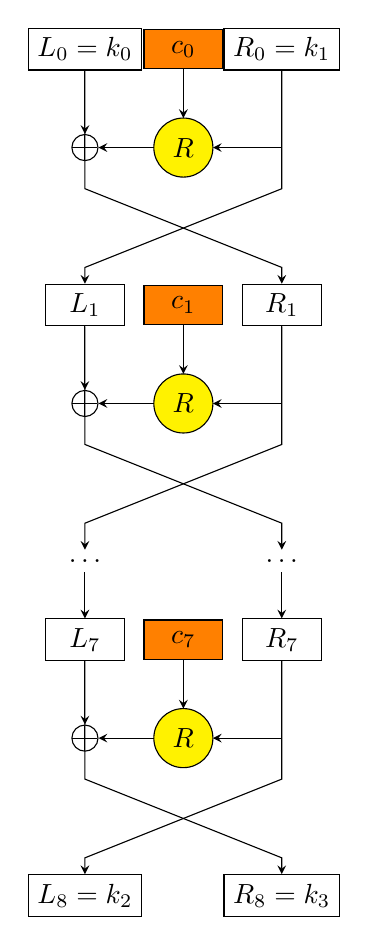
\begin{tikzpicture}[
    node distance=1.25cm
]
    %Round 1
    \node [block] (L0) {$L_0 = k_0$};
    \node [XOR, below of=L0] (x0) {};
    \node [func, right of=x0] (r0) {$R$};
    \node [right of=r0] (e0) {};
    \node [block, above of=e0] (R0) {$R_0 = k_1$};
    \node [block, above of=r0, fill=orange] (c0) {$c_0$};
    %Round 2
    \node [block, below of=x0, node distance=2cm] (L1) {$L_1$};
    \node [XOR, below of=L1] (x1) {};
    \node [func, right of=x1] (r1) {$R$};
    \node [right of=r1] (e1) {};
    \node [block, above of=e1] (R1) {$R_1$};
    \node [block, above of=r1, fill=orange] (c1) {$c_1$};
    %temp
    \node [below of=x1, node distance=2cm] (Lt) {$\ldots$};
    \node [below of=e1, node distance=2cm] (Rt) {$\ldots$};
    %Round i
    \node [block, below of=Lt, node distance=1cm] (L7) {$L_7$};
    \node [XOR, below of=L7] (x7) {};
    \node [func, right of=x7] (r7) {$R$};

    \node [right of=r7] (e7) {};
    \node [block, above of=e7] (R7) {$R_7$};
    \node [block, above of=r7, fill=orange] (c7) {$c_7$};
    %Ciphertext
    \node [block, below of=x7, node distance=2cm] (L8) {$L_8=k_2$};
    \node [block, below of=e7, node distance=2cm] (R8) {$R_8=k_3$};

    \draw [-stealth] (L0) -- (x0);
    \draw [stealth-] (x0) -- (r0);
    \draw [-stealth] (c0) -- (r0);
    \draw [-stealth] (R0) |- (r0);
    \draw [-stealth] (R0.south) -- ++(0, -1.5) 
            -- ++(-2.5, -1) -| (L1.north);
    \draw [-stealth] (L0.south) -- ++(0, -1.5)
            -- ++(2.5, -1) -| (R1.north);

    \draw [-stealth] (L1) -- (x1);
    \draw [stealth-] (x1) -- (r1);
    \draw [-stealth] (c1) -- (r1);
    \draw [-stealth] (R1) |- (r1);
    \draw [-stealth] (L1.south) -- ++(0, -1.5)
            -- ++(2.5, -1) -| (Rt.north);
    \draw [-stealth] (R1.south) -- ++(0, -1.5)
           -- ++(-2.5, -1) -| (Lt.north);

    \draw [-stealth] (Lt) -- (L7);
    \draw [-stealth] (Rt) -- (R7);

    \draw [-stealth] (L7) -- (x7);
    \draw [stealth-] (x7) -- (r7);
    \draw [-stealth] (c7) -- (r7);
    \draw [-stealth] (R7) |- (r7);
    \draw [-stealth] (L7.south) -- ++(0, -1.5)
            -- ++(2.5, -1) -| (R8.north);
    \draw [-stealth] (R7.south) -- ++(0, -1.5)
           -- ++(-2.5, -1) -| (L8.north);
\end{tikzpicture}
\end{document}